\scanpage{82}

§. \uline{Inégalités de convexité et degrés remarquables d'opérateurs, compacts}

\deleted{\unsure{La méthode de convexité}} \inserted{\textcircled{\scriptsize Th. 1}} \textcircled{1°} \deleted{\uline{Lemme fondamental}} \inserted{(H. Weyl).} Considérons deux suites finies
$(\alpha_i)_{1\leq i\leq n}$ et $(\beta_i)_{1\leq i\leq n}$ de nbs réels \inserted{on suppose} \deleted{la deuxième \unsure{décroissante}}

{\reversemarginpar\margin{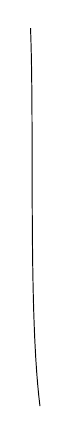
\begin{tikzpicture}[x=1cm,y=1cm]\draw[line width=.35pt] (0,0) .. controls (.05,-1.3) and (-.03,-3.6) .. (.12,-4.8);\end{tikzpicture}}}
\[
\begin{array}{@{}l@{\qquad}l@{}}
(1)&\displaystyle\boxed{\alpha_1\geq\alpha_2\mathord{.}\,\mathord{-}\,\mathord{-}\geq\alpha_n}\quad\text{et}\\
\text{\textcircled{2}}&\displaystyle\boxed{\boxed{\alpha_1+\mathord{-}\,\mathord{-}+\alpha_M\leq\beta_1+\mathord{-}+\beta_M\enspace\text{pour }M=1,\mathord{-}\,\mathord{-}n.}}
\end{array}
\]

Soit $\varphi(t_1,\mathord{-}\,\mathord{-}t_n)$ une fonction numérique \uline{convexe} et \uline{symétrique} sur $R^n$. On suppose vérifiée l'une des deux conditions suivantes : a) $\varphi$ est croissante \deleted{\unsure{(pour}}\inserted{en chaque argument $t_i$} \deleted{la \unsure{relation d'ordre naturelle|restriction d'un ensemble} sur $R^n$} b) $\sum_{i=1}^n\alpha_i=\sum_{i=1}^{n}\beta_i$.

{\reversemarginpar\margin{\begin{tikzpicture}[overlay,x=1cm,y=1cm]\draw[line width=.25pt] (.8,.2) .. controls (-.35,.4) and (-.35,-2.8) .. (.4,-3.1) .. controls (1.25,-3.5) and (2.1,-1.8) .. (1.9,-.1);\end{tikzpicture}\parbox[t]{1.85cm}{\unsure{fonction} où l'on \unsure{devrait} \unsure{admettre} \unsure{H} \illegible{1} \deleted{\unsure{partie}} \unsure{un} convexe ouvert.}}}

Sous ces conditions, on a
\[
\begin{array}{@{}l@{\qquad}l@{}}
(3)&\displaystyle\varphi(\alpha_1,\mathord{.}\,\mathord{-}\,\mathord{-},\alpha_n)\leq\varphi(\beta_1,\mathord{.}\,\mathord{-}\,\mathord{-}\beta_n)
\end{array}
\]

\deleted{Appliquons \unsure{tout de suite} le \unsure{corollaire|lemme} suivant, qui \inserted{\unsure{seul nous}} \illegible{1} \unsure{pour la} \unsure{question} qui \unsure{effacerait} \illegible{1}. On en conclut immédiatement le}

\deleted{\uline{Corollaire 1}} \inserted{\textcircled{\uuline{2°}}} Soit \inserted{$f(\rho_1,\mathord{-},\rho_n)$} fonction \deleted{\uline{\unsure{continue|numérique}}} \inserted{\uline{numérique symétrique}} de $n$ arguments \deleted{\unsure{positifs}} \inserted{$\rho_i>0$}, telle que $f(e^{t_1},\mathord{-}\,\mathord{-},e^{t_n})$ soit une fonction \uline{convexe} de $(t_1,\mathord{-}\,\mathord{-}t_n)\in R^n$. Soient $(\rho_1,\mathord{-}\rho_n)$ et $(\sigma_1,\mathord{-}\,\mathord{-},\sigma_n)$ deux suites \inserted{finies} positives, telles que \deleted{\unsure{(4bis)|(Hies.)}}

{\reversemarginpar\margin{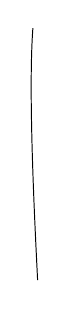
\begin{tikzpicture}[x=1cm,y=1cm]\draw[line width=.35pt] (0,0) .. controls (-.06,-.8) and (.02,-2.4) .. (.06,-3.2);\end{tikzpicture}}}
\[
\begin{array}{@{}l@{\qquad}l@{}}
\text{\textcircled{4}}&\displaystyle\boxed{\rho_1\geq\rho_2\mathord{-}\,\mathord{-}\geq\rho_n}\quad\text{et que }\deleted{\unsure{\sum\rho_i}}\\
\text{\textcircled{5}}&\displaystyle\boxed{\rho_1\mathord{.}\,\mathord{-}\rho_M\leq\sigma_1\mathord{.}\,\mathord{-}\sigma_M}\quad\text{pour }\deleted{\text{tout}}\ M=1,\mathord{-}n.
\end{array}
\]

On suppose vérifiée l'une des deux conditions suivantes :

{\reversemarginpar\margin{Il suffit que l'ensemble où est définie $f$ soit une partie \unsure{logarithmiquement} \unsure{convexe} \unsure{convenable} et symétrique.}}

a) $f$ est \inserted{définie et continue pour $\rho_i\geq0$, et} fonction croissante \deleted{des} \inserted{de} \deleted{\unsure{chacun des} $\rho_i$}\inserted{chaque argument $\unsure{\sigma_i|\rho_i}$} b) $\rho_1\mathord{.}\,\mathord{-}\rho_n=\sigma_1\mathord{-}\,\mathord{-}\sigma_n\ne0$. Sous ces conditions, on a
\[
\begin{array}{@{}l@{\qquad}l@{}}
\deleted{\unsure{(4)}}\ (6)&\displaystyle f(\rho_1,\mathord{-}\,\mathord{-}\rho_n)\leq f(\sigma_1,\mathord{.}\,\mathord{-}\sigma_n)
\end{array}
\]

En effet, si les $\rho_i,\sigma_i$ sont $>0$, cet énoncé est manifestement équivalent à l'énoncé du \deleted{lemme}\inserted{th.}, en posant $\alpha_i=\log\rho_i$, $\beta_i=\log\sigma_i$. \inserted{Cela prouve le \deleted{\unsure{corollaire}}\inserted{(2°)} en particulier dans le cas b).}

{\reversemarginpar\margin{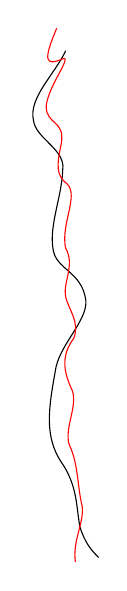
\begin{tikzpicture}[x=.0095cm,y=-.0095cm]
\draw[black] (65,37) .. controls (51,68) and (15,100) .. (22,130) .. controls (25,155) and (66,169) .. (61,197) .. controls (60,231) and (43,270) .. (48,301) .. controls (51,330) and (87,331) .. (92,371) .. controls (94,399) and (55,431) .. (51,466) .. controls (42,516) and (37,551) .. (58,585) .. controls (81,617) and (79,646) .. (84,673) .. controls (91,695) and (99,704) .. (109,714);
\draw[red] (53,7) .. controls (35,50) and (37,58) .. (61,48) .. controls (75,42) and (41,86) .. (39,111) .. controls (39,137) and (65,129) .. (59,162) .. controls (53,190) and (52,204) .. (67,215) .. controls (83,231) and (58,269) .. (65,301) .. controls (78,323) and (61,347) .. (65,366) .. controls (69,383) and (84,399) .. (76,421) .. controls (59,444) and (62,464) .. (72,487) .. controls (84,508) and (62,541) .. (70,564) .. controls (82,588) and (81,623) .. (87,645) .. controls (90,668) and (74,691) .. (78,720);
\end{tikzpicture}}}

\deleted{\unsure{On en conclut}, puisque} \inserted{Montrons que} \inserted{dans le cas a), tout} \deleted{l'ensemble des} systèmes $(\rho_i),(\sigma_i)$ tels que $\rho_i\geq0$, $\deleted{\unsure{\sigma_i\geq0|\rho_i>0}}$ \inserted{$\rho_1\geq\rho_2\mathord{-}\geq\rho_n\geq0$,} $\rho_1\mathord{.}\,\mathord{-}\mathord{.}\,\rho_M\leq\sigma_1\mathord{.}\,\mathord{-}\sigma_M$ pour $M=1,\mathord{-}\,\mathord{-}n$, \deleted{(et \unsure{éventuellement|naturellement} $\rho_1\mathord{.}\,\mathord{-}\rho_n=\sigma_1\mathord{-}\,\mathord{-}\sigma_n$)} \deleted{\unsure{est|et} l'adhérence} \inserted{est limite dans $R^{2n}$} de \deleted{sa partie formée des systèmes tels} \inserted{systèmes analogues} $(\rho'_i),(\sigma'_i)$ avec $\rho'_i>0$, $\sigma'_i>0$ (d'où résultera le \deleted{corollaire}\inserted{(2°) dans le cas a)} par prolongement par continuité). En effet, si \deleted{\unsure{les $\rho_i$}} \inserted{$\sigma_i>0$ pour tout $i$,} on voit qu'en \deleted{\unsure{tous les cas}} augmentant \inserted{de suffisamment peu} les $\rho_i$ qui seraient nuls, \deleted{\unsure{sont nuls, et il suffit d'approcher les systèmes}} on satisfait encore aux conditions imposées, \deleted{\unsure{et si} les systèmes $(\rho'_i),(\sigma'_i)$, avec $\rho'_i=\sigma'_i=\frac1n$ pour tout $i$. \unsure{D'autre part|diminuant}} d'où la conclusion \deleted{\unsure{voulue|cherchée}}\inserted{dans ce cas}.

{\reversemarginpar\margin{\unsure{{\color{red}?}}\kern-.3em\raisebox{-.7ex}{\unsure{{\color{black}?}}}}}

\deleted{Si plus généralement, \unsure{dans|donc} \illegible{1} \unsure{l'on} \illegible{2} \unsure{qui sont} \illegible{1} d'abord \illegible{1}}

{\reversemarginpar\margin{83}}
